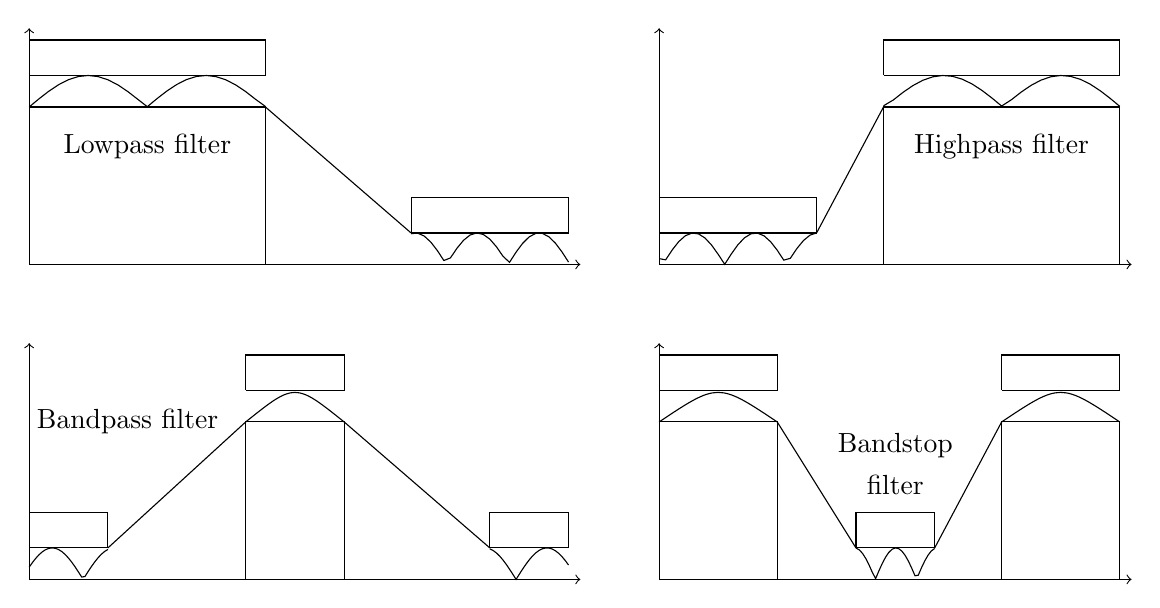
\begin{tikzpicture}
	\draw[->] (0,0) -- (0,3);
	\draw[->] (0,0) -- (7,0);
	
	\draw (0,2.4) -- (0,2.85) -- (3,2.85) -- (3,2.4) -- (0,2.4);
	\draw (0,0) -- (0,2) -- (3,2) -- (3,0) -- (0,0);
	\draw (4.85,0.4) -- (4.85,0.85) -- (6.85,0.85) -- (6.85,0.4) -- (4.85,0.4);
	
	\draw[->] (0,-4) -- (0,-1);
	\draw[->] (0,-4) -- (7,-4);
	
	\draw (0,-3.6) -- (0,-3.15) -- (1,-3.15) -- (1,-3.6) -- (0,-3.6);
	\draw (2.75,-1.6) -- (2.75,-1.15) -- (4,-1.15) -- (4,-1.6) -- (2.75,-1.6);
	\draw (2.75,-4) -- (2.75,-2) -- (4,-2) -- (4,-4) -- (2.75,-4);
	\draw (5.85,-3.6) -- (5.85,-3.15) -- (6.85,-3.15) -- (6.85,-3.6) -- (5.85,-3.6);
	
	\draw[->] (8,0) -- (8,3);
	\draw[->] (8,0) -- (14,0);
	
	\draw (8,0.4) -- (8,0.85) -- (10,0.85) -- (10,0.4) -- (8,0.4);
	\draw (10.85,2.4) -- (10.85,2.85) -- (13.85,2.85) -- (13.85,2.4) -- (10.85,2.4);
	\draw (10.85,0) -- (10.85,2) -- (13.85,2) -- (13.85,0) -- (10.85,0);
	
	\draw[->] (8,-4) -- (8,-1);
	\draw[->] (8,-4) -- (14,-4);
	
	\draw (8,-1.6) -- (8,-1.15) -- (9.5,-1.15) -- (9.5,-1.6) -- (8,-1.6);
	\draw (8,-4) -- (8,-2) -- (9.5,-2) -- (9.5,-4) -- (8,-4);
	\draw (10.5,-3.6) -- (10.5,-3.15) -- (11.5,-3.15) -- (11.5,-3.6) -- (10.5,-3.6);
	\draw (12.35,-1.6) -- (12.35,-1.15) -- (13.85,-1.15) -- (13.85,-1.6) -- (12.35,-1.6);
	\draw (12.35,-4) -- (12.35,-2) -- (13.85,-2) -- (13.85,-4) -- (12.35,-4);
	
	\draw[domain=0:3] plot (\x, {2 + abs(0.4*sin(2.1*\x r))});
	\draw (3,2) -- (4.85,0.4);
	\draw[domain=4.85:6.85] plot (\x, {abs(0.4*sin(4*(\x+0.20) r))});
	 
	\draw[domain=0:1] plot (\x, {abs(0.4*sin(4*(\x+0.10) r)) - 4});
	\draw (1,-3.6) -- (2.75,-2);
	\draw (2.75,-2) .. controls (3.375,-1.5) .. (4,-2);
	\draw (4,-2) -- (5.85,-3.6);
	\draw[domain=5.85:6.85] plot (\x, {abs(0.4*sin(4*(\x+0.10) r)) - 4});
	 
	\draw[domain=8:10] plot (\x, {abs(0.4*cos(4*(\x+0.20) r))});
	\draw (10,0.4) -- (10.85,2);
	\draw[domain=10.85:13.85] plot (\x, {2 + abs(0.4*sin(2.1*(\x+1.1) r))});
	
	\draw (8,-2) .. controls (8.75,-1.5) .. (9.5,-2);
	\draw (9.5,-2) -- (10.5,-3.6);
	\draw[domain=10.5:11.5] plot (\x, {abs(0.4*sin(6*(\x+0.25) r)) - 4});
	\draw (11.5,-3.6) -- (12.35,-2);
	\draw (12.35,-2) .. controls (13.1,-1.5) .. (13.85,-2);
	
	\draw (1.5,1.5) node {Lowpass filter};
	\draw (12.35,1.5) node {Highpass filter};
	\draw (1.25,-2) node {Bandpass filter};
	\draw (11,-2.3) node {Bandstop};
	\draw (11,-2.8) node {filter};
\end{tikzpicture}